% ~~~~~~~~~~~~~~~~~~~~~~~~~~~~~~~~~~~~~~~~~~~~~~~~~~~~~~~~~~~~~~~~~~~~~~~~~~~~~
%                                 BACKGROUND
% ~~~~~~~~~~~~~~~~~~~~~~~~~~~~~~~~~~~~~~~~~~~~~~~~~~~~~~~~~~~~~~~~~~~~~~~~~~~~~
\chapter{Background}\label{chap:2}
  \lhead{Chapter 2. \emph{Background}}
  In this chapter, there will be introduced Python programming language and
different existing approaches in solving board games with agent based model.

\section{Python}
Python is widely used and popular
programming language. It is an interpreted, high-level, dynamic programming
language supporting multiple programming paradigms, including functional,
object-oriented and procedural style. It has been designed with regard to
readability, easy adoption for novices and scalability of programs. Python
offers a lot of utilities as part of its comprehensive standard library. It is
possible to work in Python under multiple operating systems and it is often
standard component among many linux distributions. Main reasons why I chose
Python was that I had four years of experience with it and for its
maintainability.

\section{Agent based model, Markov decision process and Game theory}
Agent based model (ABM) is a paradigm in modeling systems comprised
of autonomous agents. Also, it is a class of computational models for
simulations of the actions and interactions between agents. Althought, there
are multiple definitions of what is considered agent \cite{abm}, often, agent
is an identifiable component with reaction rules able to make independent
decisions (or behaviours) and sometimes with ability to learn and adapt to
the environment.

Markov decision process (MDP) is a mathematical model for describing stochastic
discrete time decision processes. Important property that the proccess must
have is a memorlylessness, which means that the next state depends only
on current state and not on any other preceeding states.

Game theory studies conflict or cooperation between rational decision makers
and also different strategies for given problems. Knowledge from computational
complexity theory is used to determine or estimate game complexity. Here, MDP
is often used to describe such rational decision makers.

When trying to find the optimal strategy where due to the large number
of states in a game it is not feasible to use brute-force, there are often
used:
\begin{itemize}
  \vspace*{-0.25cm}
  \setlength\itemsep{0cm}
  \item Heuristic methods - Minimax, Alpha-beta pruning
  \item Reinforcement learning (RL) - Monte-carlo algorithms,
                                      Temporal difference methods, Q-learning
  \item Evolutionary methods - genetic algorithm
  \item Artificial neural networks combined with RL methods
  \vspace*{-0.15cm}
\end{itemize}

\section{Minimax}
The principle of the algorithm is to find the best action for an agent by
traversing a game tree while minimizing maximum possible losses.
The requirement for the algorithm to work is existance of a function capable to
evaluate arbitrary position in the game. Also, it is assumed that there are no
infinite sequences of positions allowed.

Algorithm walks througt all the possible moves, performs heuristic evaluation
of subsequent positions and picks up the action bringing the most advantageous
position. Evaluation is can be done by static evaluation funciton or the same
algorithm is executed recursively for the opponent. Often, recursion has
limited depth to ensure the algorithm ends in a reasonable time.

\section{Alpha-beta pruning}
\begin{wrapfigure}{r}{0.5\textwidth}
  \vspace*{-2.85cm}
  \centering
  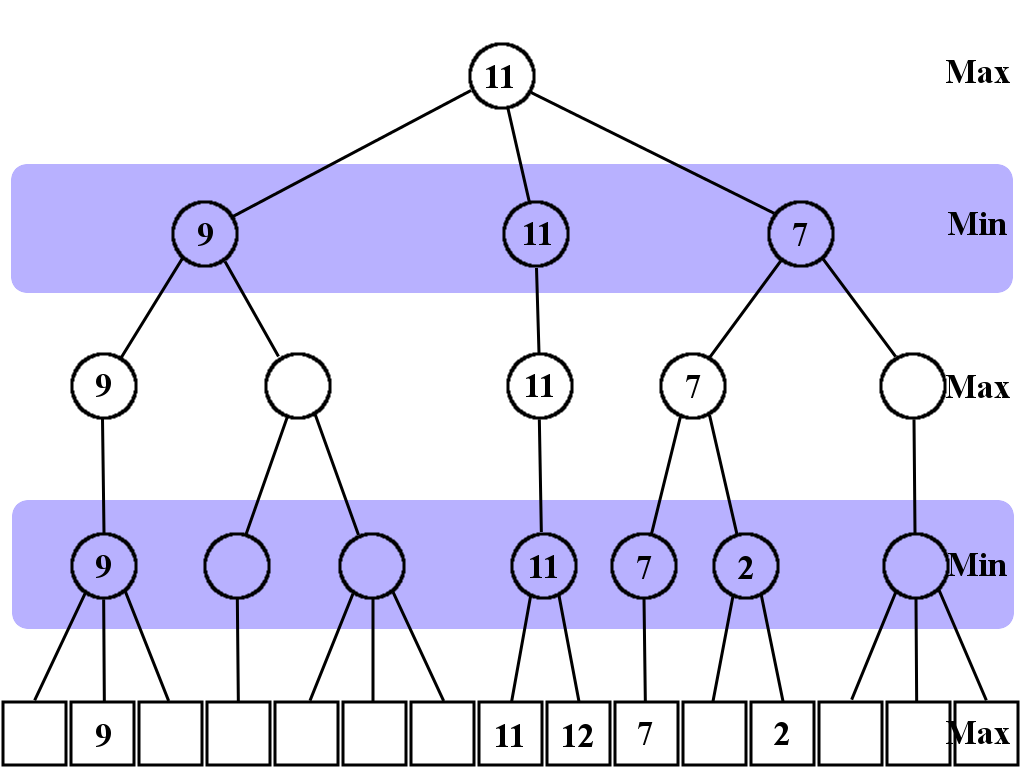
\includegraphics[width=0.5\textwidth]{alpha-beta_tree2.png}
  \vspace*{-0.85cm}
  \caption{alpha-beta pruning}
  \label{fig:abp}
  \vspace*{-0.60cm}
\end{wrapfigure}

Alpha-beta pruning is enhancement of minimax algorithm. On average, it
speeds up the minimax algorithm by eliminating branches of a game tree which
will be certainly left off from choosing. Initially, alpha is set to negative
infinity and beta to positive infinity. When there is a node evaluated, where
maximizing player is sure to have the same or more than player choosing
minimum is certain to have ($\alpha{=>}\beta$), all subsequent branches will
not be explored, since it would make outcome on the parent node worse.


In example scenario from figure \ref{fig:abp}, middle branch has been evaluated
first, where minimizing player chose $11$. This has been back-propagated
to the top node as $\alpha{>=}11$. Next, right branch evaluated ended up in the
leave with value $2$. Minimizing parent branch is then assured to have minimum
of $\beta{<=}2$, which is certainly less than maximizing top node can choose
from, so the other leaf is not explored. Then, exploration gets to leaf node
with value 7, which is back-propagated to the uppermost minimizing player.
Since his $\beta{<=}7$ other branches are left off because root node would not
pick this branch having $11$ as a better choice. At last, exploration ends up
in the leaf with value $9$. Minimizing parent node is now certain to have
$\beta{<=}9$ while $\alpha{>}\beta$, therefore, other nodes are not explored.
Value $9$ is back-propagated through the parent maximizing to the uppermost
$\beta$ value and so, this whole branch is cut off from further exploration.
Since, there are no other branches to explore for the root maximizing player,
maximum value $11$ is chosen as a result.

In the end, 15 out of 31 nodes were not explored. With higher branching factor,
it could be even better ratio in the best case scenario. Despite that
alpha-beta pruning may be improvement to minimax, with its exponential
time complexity it is less likely to be used for problems, where there is no
well known evaluation function for that particular problem.


\section{Reinforcement Learning}
TODO

\section{Q-Learning}
Q-Learning is reinforcement learning method. It learns an action-value
(q-value) function for any finite Markov decision process used to find
optimal policy for the agent. After it has learned the q-value function,
it can follow the optimal strategy by choosing best q-value. ?citation?
Algorithm is value iteration update for every observed state ?citation?:
\begin{equation}
Q_{t+1} \leftarrow Q_t(s_t, a_t) + \alpha \cdot (
    R_{t+1} + \gamma\cdot {\max_a}\,Q_t(s_{t+1}, a) - Q_t(s_t, a_t)
)
\end{equation}
where $Q_t(s_t, a_t)$ is old value, $\alpha$ is learning rate, $R_{t+1}$ is
reward after performing action $a_t$ in state $s_t$, $\gamma$ is discount
factor and $\underset{a}{\max}\,Q_t(s_{t+1}, a)$ is maximum optimal future
value.

\section{Evolution methods and genetic algorithms}
TODO

\section{Perceptron}
\begin{wrapfigure}{r}{0.4\textwidth}
  \vspace*{-1.85cm}
  \centering
  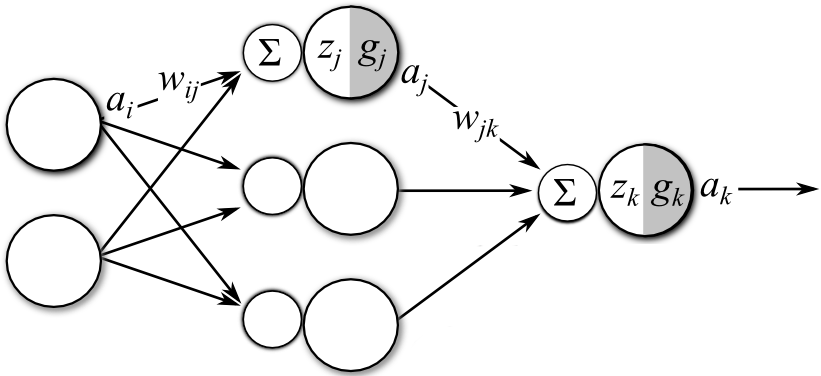
\includegraphics[width=0.4\textwidth]{perceptron.png}
  \vspace*{-0.85cm}
  \caption{ANN}
  \label{fig:network}
  \vspace*{-0.60cm}
\end{wrapfigure}

Artifitial neural network (ANN) is a family of models inspired by biological
neural networks used in computer science to approximate functions with
large number of inputs. Generally, artifitial neural network is presented
as a system of interconnected neurons exchanging messages between each
other. These connections have weights that can be adjusted based on
experience which makes the network capable of learning.

Perceptron is an algorithm for supervised learning of binary classifiers
where one neuron has multiple weighted inputs and single output. Single
perceptron can learn to decide between two linearly separable
classes. Multiple perceptrons in multiple layers (MLP) use arbitrary
activation function which makes it able to perform classification or
regression based on the activation function chosen.

\section{Perceptron estimating Q-values}
\begin{wrapfigure}{r}{0.42\textwidth}
  \vspace*{-1.15cm}
  \begin{equation}
    \label{eqn:otheloqupdate}
    \hat{Q}^{new}\!\leftarrow\!r_t\!+\!{\gamma}{\max_a}\,\hat{Q}(s_{t+1},\!a)
    % \hat{Q}_t^{new}
    % \leftarrow r_t + {\gamma}{\max_a}\,\hat{Q}_{t+1}(s_{t+1}, a)
  \end{equation}
  \vspace*{-0.95cm}
\end{wrapfigure}

Main advantage of ANN is its ability to generalize. This is has been used
in game othello \cite{othello} with combining Q-learning so that network
has learned to estimate q-values for each state. Learning rate $\alpha$ has
not been directly used in iteration update (\ref{eqn:otheloqupdate}) since
ANN has also learning rate so it can be adjusted there.

